% Thesis section draft (Week 18). Self-contained; compile inside the thesis preamble (amsmath, booktabs, graphicx).
% Numbers are copied from outputs/week18_independent_research/round_1/ and round_2/ (decision.json, contrasts.csv).
\section{Learning the level set of the observed melt-pool depth}
\label{sec:depth-level-set}

\subsection{Motivation: the regime label is a thresholded continuous output}
Every paid simulation returns more than its regime label. On the 405 OLD simulations, the binary label
\texttt{has\_keyhole} coincides with a threshold of the maximum melt-pool depth: all Keyhole runs have
$d_{\max}\ge 111.2\,\mu$m and all others $d_{\max}\le 111.6\,\mu$m (AUC $1.000$, best single-threshold balanced
accuracy $0.9985$). A binary Gaussian-process classifier therefore discards most of what a query reveals. Away from
the boundary, a label is nearly certain under the current model and carries almost no information about the latent
function, whereas the depth is observed everywhere on the conduction side.

\subsection{Method}
Let $t(x)=\log d_{\max}(x)$ for inputs $x=(P,V_X,L_S,S_T)$. We place a Gaussian-process prior on $t$ (ARD Matérn-$3/2$
kernel on standardized log inputs, white noise, hyperparameters by type-II maximum likelihood after every query) and
estimate the regime boundary as the level set $\{t(x)=\log u\}$. The depth threshold $u$ is learned online from the
revealed (depth, label) pairs: the midpoint of the gap between the deepest conduction run and the shallowest Keyhole run
when they separate, otherwise a one-dimensional logistic fit. The Keyhole probability is
$\Phi\big((\mu(x)-\log u)/s(x)\big)$ with posterior mean $\mu$ and standard deviation $s$. Queries follow the straddle
rule $\arg\max_x\,1.96\,s(x)-|\mu(x)-\log u|$. Startup is identical to the binary reference (eight maximin points plus
maximin continuation until both classes are observed). The formulation was proposed in Week~7; here it is evaluated on
a redesigned benchmark under a pre-registered protocol.

\paragraph{Why it should help (information per query).} With a probit link and latent margin $m$ (in noise units),
one binary label carries Fisher information
\begin{equation}
  I_{\mathrm{bin}}(m)=\frac{\varphi(m)^2}{\Phi(m)\,\Phi(-m)}\,,\qquad I_{\mathrm{bin}}(0)=0.637,\; I_{\mathrm{bin}}(2)=0.131,\; I_{\mathrm{bin}}(3)=0.015,
\end{equation}
about the latent at the queried point, whereas an observed depth with noise $\sigma$ carries $1/\sigma^2$ whatever its
distance from the boundary. The prediction is that the gain concentrates at small budgets and in conduction-rich
pools. A one-dimensional analysis shows that censored continuous observations shorten threshold search only on fine
pools; on our coarse four-dimensional pools any gain must therefore come from depth information shared across the
boundary surface.

\subsection{Protocol}
Development used only repeats 1--8 of the locked benchmark and digital-twin seeds 0--7. The candidate, reference,
data blocks, endpoints, decision rule and predictions were frozen and pushed before the confirmation run (round~1,
commit \texttt{fc1afb50}). Confirmation used the untouched block C1 (repeats 9--12) and fresh twin seeds 100--107.
The reference is G3 with probability-margin acquisition. Endpoints: balanced-accuracy area under the learning curve
(BA AULC) over the budget grid, the number of paid simulations needed to reach the reference's mean accuracy at 80
queries (queries-to-target), the historical q20 accuracy, and, on twins, the normalized surface distance (NSD, $\tau=0.1$).
Intervals are 95\% bootstrap intervals over repeats. All Laplace and GP fits were checked for convergence (no fit with
fixed-point error above $10^{-6}$).

\subsection{Results}
\begin{table}[h]
\centering
\caption{Round-1 confirmation (block C1; fresh twin seeds). Differences are depth GP + straddle minus G3 + margin.}
\label{tab:depth-round1}
\begin{tabular}{llrl}
\toprule
Task & Endpoint & Difference & 95\% interval \\
\midrule
R3\_OLD (primary) & BA AULC & $+0.0285$ & $[+0.010,\,+0.047]$ \\
R3\_OLD & simulations to G3's B80 accuracy & $30$ vs $88$ ($-66\%$) & $[44\%,\,74\%]$ \\
R3\_OLD & q20 AULC & $-0.003$ & $[-0.031,\,+0.026]$ \\
R2rev (OLD pool, NEW prior) & BA AULC & $+0.012$ & $[-0.001,\,+0.024]$ \\
Twin T\_DEPTH (primary) & NSD AULC & $+0.082$ & $[+0.041,\,+0.125]$ \\
Twin T\_TOBIT, OLD inputs & NSD AULC & $+0.062$ & $[+0.028,\,+0.104]$ \\
Twin T\_TOBIT, NEW-like inputs & NSD AULC & $+0.009$ & $[-0.000,\,+0.021]$ \\
\bottomrule
\end{tabular}
\end{table}
All three pre-registered success routes held and the candidate was non-inferior on every in-scope task. The gain is
largest early: on R3\_OLD the depth model reaches a balanced accuracy of $0.927$ after 24 simulations, against $0.863$
for the binary reference (Figure~\ref{fig:depth-round1}). In six depth stress worlds (fresh seeds) no world fell below
the frozen limit of $-0.03$ NSD AULC. The gain vanished only under 25\% multiplicative depth noise
($-0.018$, $[-0.077, 0.034]$). It persisted under a threshold that drifts by $\pm15\%$ across the input space
($+0.052$) and when 30\% of the runs report no depth ($+0.033$).

\begin{figure}[h]
\centering
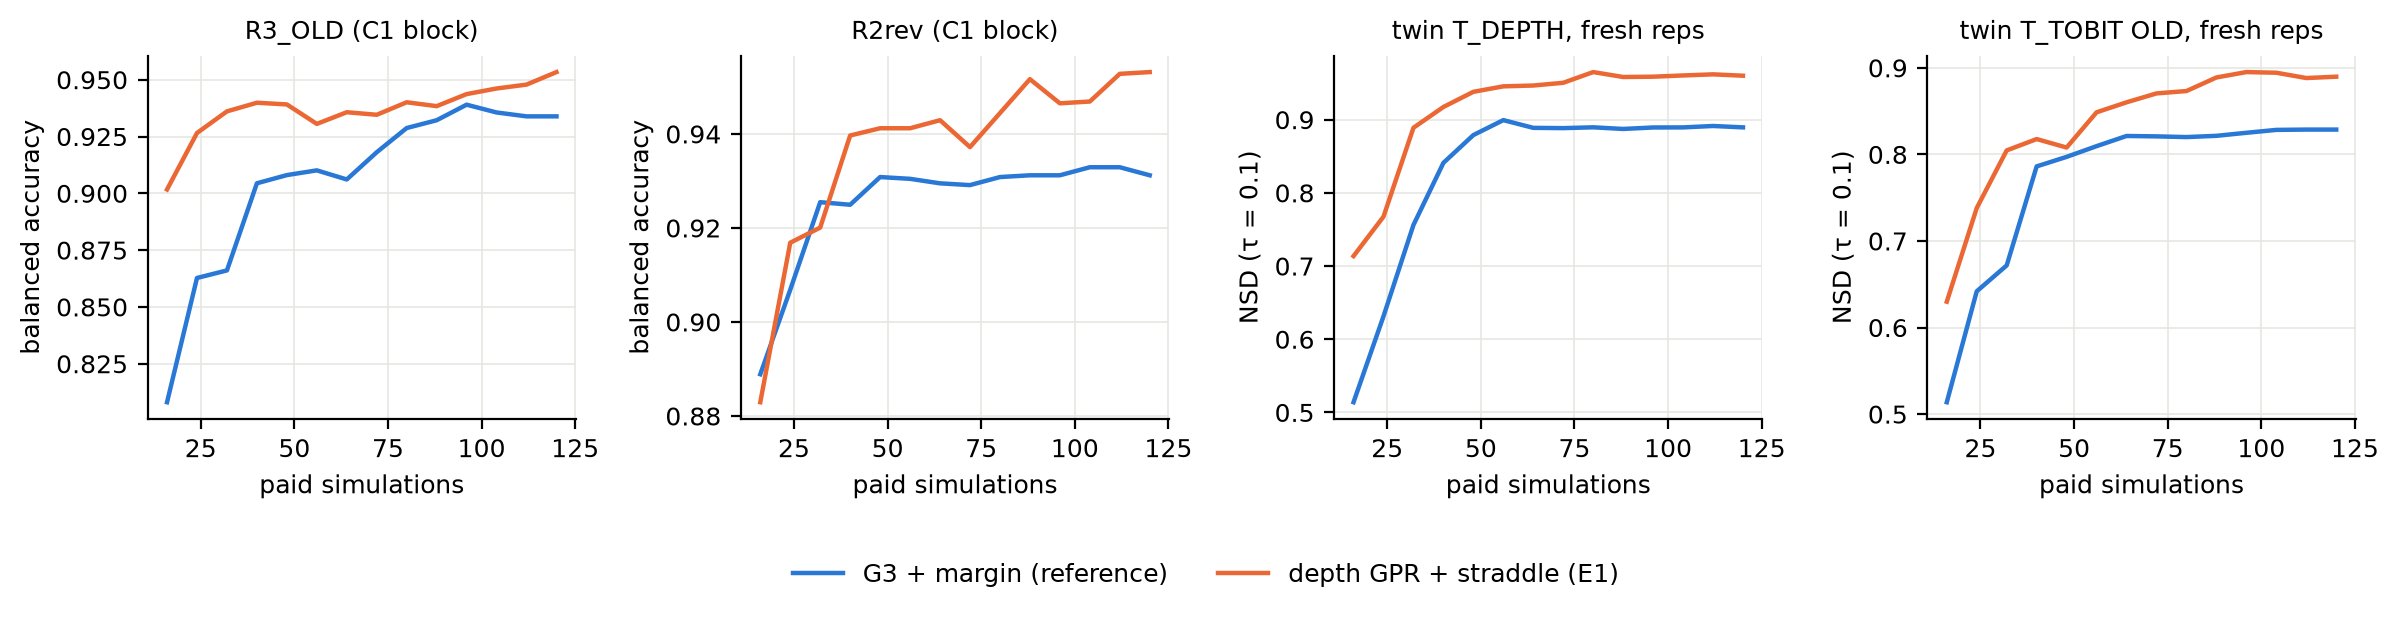
\includegraphics[width=\textwidth]{fig_w18_round1_confirmation.png}
\caption{Learning curves in the round-1 confirmation: real OLD tasks (block C1) and digital twins (fresh seeds).}
\label{fig:depth-round1}
\end{figure}

\subsection{Scope: what happens on the NEW campaign}
The NEW monitors were obtained only after round~1. With them, the NEW label turns out \emph{not} to be a max-depth
threshold: AUC $0.891$; 7 of the 12 non-Keyhole NEW runs exceed $111\,\mu$m, almost all of them fast scans
($V_X>0.85$\,m/s) whose depth peaks transiently early in the run. The depth model assumes a single depth threshold,
and this assumption fails on NEW. On the development repeats, with depth available for every run, its advantage
disappears on the pooled task ($-0.001$, $[-0.004, 0.003]$) and turns negative on NEW alone ($-0.021$,
$[-0.080, 0.039]$). A second pre-registered round on block C2 (commit \texttt{1d560792}) tested this scope question and the
replication of the OLD result. With depth for every run, the pooled task showed no gain ($+0.004$, $[-0.001, 0.009]$) and NEW showed a loss
($-0.022$, $[-0.070, 0.030]$). On R3\_OLD the gain replicated in direction but was smaller
($+0.016$, $[0.013, 0.020]$; 12\% fewer simulations to the reference's B80 accuracy). That is below the
pre-registered bar of $+0.02$. Across the three independent repeat blocks of R3\_OLD the estimates are $+0.021$ (development),
$+0.029$ (C1) and $+0.016$ (C2), all with intervals above zero.

\subsection{Limitations}
(i) The historical q20 endpoint, which weighs the 20\% of test points nearest the observed boundary, does not improve:
it is lower on R2rev (C1) and on R3\_OLD in C2 ($-0.028$, $[-0.046, -0.017]$). The depth model trades accuracy close to
the boundary for accuracy elsewhere and in the rare class. (ii) The method is fragile to stale hyperparameters: refitting the GP only every eight queries
turned a $+0.012$ gain into $-0.081$ on R2rev during development. (iii) The real confirmation uses split
confirmation on data seen in earlier weeks; the digital twins are fitted to the same OLD depth. (iv) With partial
depth (some runs reporting only the label) the method is worse than the binary reference, because its queries on
label-only points are wasted.

\subsection{Conclusion}
When the simulator's continuous output is observed and the label is a threshold of that output, learning the level
set of the output is consistently more sample-efficient than learning the binary label. The gain in balanced-accuracy
AULC is $+0.016$ to $+0.029$ across three repeat blocks, and it is concentrated at small budgets. Where the label is
not a threshold of the observed output, as for the fast NEW scans, the binary G3 + margin procedure remains the method
of choice.
